\subsection{Previous Work}\label{sec:Research:Viz:ACA}
The original simulation\cite{modules:CS257Coursework} included a simple image visualizer for a static state, which evaluated one of two quantities over the grid and produced a \texttt{.ppm} image with the result.
These quantities were Vorticity ($\zeta$), the strength of vortical (a.k.a. rotational) motion at each point in the grid; and Stream Function ($\psi$), the contours of which define streamlines.
Streamlines are lines that are parallel to the velocity vector at each point, allowing the long-term flow of particles to be represented with a single line, and thus in a static image.\cite{NASADefinitionStreamlines}
The quantities are defined by \cref{eq:zeta,eq:vorticity}, as specified in \cite{book:griebel1998numerical}.
Examples of these modes are shown in \cref{fig:ppms}.

\begin{equation}
    \zeta(x,y) := \frac{\delta{u}}{\delta{y}} - \frac{\delta{v}}{\delta{x}}
    \label{eq:zeta}
\end{equation}
\begin{equation}
    \frac{\delta{\psi}(x,y)}{\delta{x}} := -v,\quad \frac{\delta{\psi}(x,y)}{\delta{y}} := u
    \label{eq:vorticity}
\end{equation}

\begin{figure}[ht]
    \centering
    \subcaptionbox{Vorticity $\zeta$\label{fig:zeta_ppm}%
    }[\linewidth]{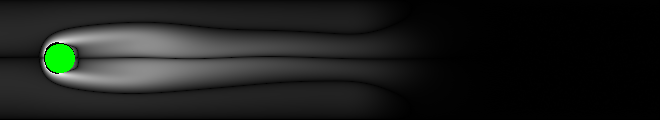
\includegraphics[width=\linewidth,natwidth=660,natheight=120]{Ch20Research/figures/output_zeta.png}
    }
    
    \subcaptionbox{Stream Function $\psi$\label{fig:psi_ppm}%
    }[\linewidth]{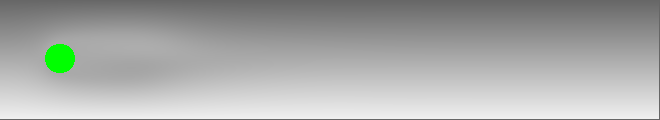
\includegraphics[width=\linewidth,natwidth=660,natheight=120]{Ch20Research/figures/output_psi.png}
    }
    
    \subcaptionbox{Pressure $p$\label{fig:pressure_ppm}%
    }[\linewidth]{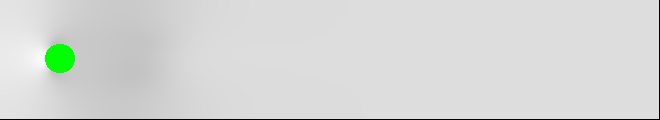
\includegraphics[width=\linewidth,natwidth=660,natheight=120]{Ch20Research/figures/output_pressure.png}
    }
    \caption{Examples of the three outputs available from the original visualization.}%\\These all visualize the output of a modified ACA coursework running for 10 seconds on the provided input data.
    %  all visualizing the same state.
    \label{fig:ppms}
\end{figure}
% Criticism of zeta, psi, pressure implementation
The vorticity image in \cref{fig:zeta_ppm} competently shows which areas of the grid contain particle movement.
However near the edges of the obstacle circle (shown in green) the edges are black, implying no movement or rotation, which is incorrect and also a distracting artifact for the viewer.
These are due to the imprecise nature of the original code, which only uses the differences to the East and South to find $\zeta$.
This breaks down when the squares in these directions are boundaries, and the program defaults to zero.
A better solution would be to take the central difference whenever possible, and to fall back to using only one side when adjacent to an boundaries.
This would mean the only points where this breaks down are where a square is surrounded by boundaries on opposite sides, which is much less likely and would also likely break other areas of the simulation.

The Stream Function visualization (\cref{fig:psi_ppm}) is nearly impossible to visually parse, which makes sense as the velocity information is encoded in the differences between adjacent squares and not directly in the colors.
The Stream Function is not intended to be directly visualized, but instead used to find streamlines which can be visualized directly.

\label{sec:VizPressureCritique}
During program development a third mode was added which directly visualized the pressure values to aid in debugging, but this was not a very useful visualization as seen in \cref{fig:pressure_ppm}.
Pressure is only ever referenced in the Navier-Stokes equation (and subsequently the algorithm) as a relative value.
However, the simulation in practice ends up increasing all cells by a small amount each iteration.
This overall increase in pressure values is ignored by the simulation, but the visualization doesn't adjust for it.
In this example, the pressure values have all increased so even the lowest pressure value is a mid-gray.
If the program simulated for too long, the pressure values would become too high and the visualization would be entirely white.
This should be accounted for in the visualization, but also implies the base simulation is unstable.
The simulation stability will be touched on in Results/Evaluation (\cref{sec:Results,sec:Evaluation}).